% SVN info for this file
\svnidlong
{$HeadURL$}
{$LastChangedDate$}
{$LastChangedRevision$}
{$LastChangedBy$}

\chapter{Integrali dipendenti da un parametro}
\labelChapter{integralidipendentiparametro}

\begin{introduction}
	‘‘La matematica confronta i più disparati fenomeni e scopre le analogie segrete che li uniscono.''
	\begin{flushright}
		\textsc{Joseph Fourier,} cercando disperatamente di motivare ai suoi genitori la scelta di studiare matematica.
	\end{flushright}
\end{introduction}
\lettrine[findent=1pt, nindent=0pt]{S}{i} sa, molti quesiti matematici sono particolarmente difficili da risolvere, anche solo per la loro complessità computazionale. Questo è un problema soprattutto nel mondo applicativo-ingegneristico, dove spesso è importante avere dei metodi risolutivi che siano anche pratici da implementare in \textit{macchina}.\\
Per fare un esempio pratico, sappiamo che un \textit{suono} si può descrivere come la somma di diverse \textit{sinusoidi} a frequenze e ampiezze differenti: ma come possiamo trovare da un rumore qualunque le sinusoidi che lo generano?\\
Per ‘‘aggirare'' questi inconvenienti si fa uso di quelle che sono chiamate \textit{trasformate integrali}, operazioni che mappano funzioni dal loro dominio originale in un altro dominio, dove può essere molto più facile risolvere il problema che nel dominio originale; per fare questo cambio è necessario integrare una funzione a \textit{due} variabili, di cui una è la vecchia variabile e fungerà da \textit{variabile di integrazione}, mentre quella nuova - che rispetto all'integrale non è altre che un \textit{parametro} - è detta di \textit{trasformazione} e ci permetterà il passaggio al nuovo dominio; in altre parole, ci serve trattare gli \textbf{integrali dipendenti da un parametro}.\\
Già nel corso di \textsc{Analisi Matematica 2} li abbiamo incontrati nella teoria dell'integrazione di Riemann; in questo capitolo espanderemo questo argomento agli \textit{integrali di Lebesgue}, in modo da poter trattare anche funzioni complesse e studiare \textit{continuità} e \textit{derivabilità} con gli strumenti visti nei precedenti capitoli. Concluderemo introducendo una delle trasformazioni più importanti per la matematica teorica e applicata, le \textbf{trasformate di Fourier} - anche se non andremo nei dettagli delle loro vaste e innumerevoli applicazioni, preferendo lasciare alcune riferimenti a fine capitolo per approfondimento.\newpage
\section{Integrali dipendenti da un parametro}
\begin{define}[Integrali dipendenti da un parametro]
	Consideriamo lo spazio di misura $\left(\realset,\mathcal{L}\left(\realset\right),m_1\right)$. Un \textbf{integrale dipendente da un parametro}\index{integrale!dipendente da un parametro} è una funzione
	\begin{equation}
		F(t)=\int_I\mvf{f}{t}{x}dm_1(x),\ \forall t\in J
	\end{equation}
	dove $I,J$ sono intervalli in $\realset$ e
	\begin{equation*}
		\funztot{f}{I\times J}{\complexset}{\left(t,x\right)}{\mvf{f}{t}{x}}
	\end{equation*}
	è tale per cui $\forall t\in I\ \funz{f\left(t,\cdot\right)}{J}{\complexset}$ integrabile.
\end{define}
Vogliamo studiare le proprietà di continuità e derivabilità dell'integrale dipendente da una parametro a partire da quelle della funzione $f$ che lo definisce.
\begin{theorema}[Teorema di continuità e derivabilità di integrali dipendenti da un parametro]
	Siano $I,J\subseteq\realset$ intervalli e sia $\funz{f}{I\times J}{\complexset}$ tale che $f\left(t,\cdot\right)$ sia integrabile, $\forall t\in I$, così da poter definire $F$. Consideriamo
	\begin{equation*}
		F(t)=\int_I\mvf{f}{t}{x}dm_1(x)
	\end{equation*}
	\begin{enumerate}
		\item Se
		\begin{itemize}
			\item $f\left(\cdot, x\right)$ è continua su $I$, $\forall x\in J$.
			\item $\exists \funz{\phi}{I}{\realset}$ integrabile tale che
			\begin{equation*}
				\abs{\mvf{f}{t}{x}}\leq\phi(x),\ \forall \left(t,x\right)\in I\times J
			\end{equation*}
		\end{itemize}
		allora $F$ è continua su $I$.
		\item Se
		\begin{itemize}
			\item $\exists\frac{\partial f}{\partial t}$ su $I\times J$.
			\item $\exists\funz{\psi}{J}{\realset}$ integrabile tale che
			\begin{equation*}
				\abs{\frac{\partial f}{\partial t}\left(t,x\right)}\leq\psi(x),\ \forall \left(t,x\right)\in I\times J
			\end{equation*}
			allora $F$ è derivabile su $I$ e si ha la \textbf{derivazione sotto segno di integrale}\index{derivazione sotto segno di integrale}:
			\begin{equation*}
				F'(t)=\int_J\frac{\partial f}{\partial t}\left(t,x\right)dm_1(x), \forall t\in I
			\end{equation*}
		\end{itemize}
	\end{enumerate}
\end{theorema}
Per dimostrare questo teorema ci serviranno i seguenti fatti:
\begin{itemize}
	\item \textbf{Teorema di relazione:} data $\funz{g}{I\subseteq\realset}{\complexset}$ e $\overline{t}\in I$, si ha
	\begin{equation}
		\lim_{t\to\overline{t}}g(t)=L\in\complexset\iff\lim_{n\to+\infty}g\left(t_n\right)=L,\ \forall t_n\to\overline{t}
	\end{equation} cioé $g$ converge a $L$ lungo \textit{tutte} le possibili successioni $t_n$ convergenti a $\overline{t}$.
	\item \textbf{Teorema di Lagrange:} data $\funz{g}{I\subseteq\realset}{\complexset}$ derivabile su $I$, si ha
	\begin{equation}
		\forall t_1,t_2\in I, \abs{g\left(t_1\right)-g\left(t_2\right)}\leq \bigg(\sup_{t\in\left[t_1,t_2\right]}\abs{g'(t)} \bigg)\abs{t_1-t_2}
	\end{equation}
\end{itemize}
\begin{demonstrationcaputwt}[della continuità e derivabilità di {$F$}]~
	\begin{enumerate}[label=\Roman*]
		\item Dobbiamo provare che
		\begin{equation*}
			\forall \overline{t}\in I,\ \lim_{t\to\overline{t}}F(t)=F\left(\overline{t}\right)
		\end{equation*}
		È sufficiente provare che, per il primo fatto enunciato precedentemente,
		\begin{equation*}
			\forall \overline{t}\in I,\ \forall t_n\to\overline{t}, \lim_{n\to+\infty}F\left(t_n\right)=F\left(\overline{t}\right)
		\end{equation*}
		Siano quindi $\overline{t}\in I$ e $t_n\to\overline{t}$ fissati: dobbiamo provare che
		\begin{equation*}
			\lim_{n\to+\infty}\int_Jf\left(t_n,x\right)dm_1(x)=\int_Jf\left(\overline{t},x\right)dm_1(x)
		\end{equation*}
		Ponendo
		\begin{align*}
			g_n(x)\coloneqq f\left(t_n,x\right)\\
			\overline{g}(x)\coloneqq f\left(\overline{t},x\right)
		\end{align*}
		allora la relazione da provare si scrive come
		\begin{equation*}
			\lim_{n\to+\infty}\int_Jg_n(x)dm_1(x)=\int_J\overline{g}(x)dm_1(x)
		\end{equation*}
		ossia ho ottenuto un problema di passaggio al limite sotto segno di integrale. Applichiamo il teorema di convergenza dominata, verificandone le ipotesi:
		\begin{itemize}
			\item \textbf{Convergenza puntuale:}
			\begin{equation*}
				\forall x\in J,\ \lim_{n\to+\infty}g_n(x)=\lim_{n\to+\infty}f\left(t_n,x\right)=f\left(\overline{t},x\right)=\overline{g}(x)
			\end{equation*}
			perché $f\left(\cdot,x\right)$ è continua rispetto alla $t$.
			\item \textbf{Maggiorazione (convergenza dominata):}
			\begin{equation*}
				\abs{g_n(x)}\underset{\substack{\forall n\geq 1\\\forall x\in J}}{=}\abs{f\left(t_n,x\right)}\leq \phi(x)\quad\text{(indipendentemente da $n$)}
			\end{equation*}
		\end{itemize}
		Si può allora passare al limite sotto segno di integrale e concludere.
		\item Dobbiamo provare che
		\begin{equation*}
			F'(t)=\int_J\frac{\partial f}{\partial t}\left(\overline{t},x\right)dm_1(x),\ \forall \overline{t}\in I
		\end{equation*}
		ossia
		\begin{equation*}
			\lim_{t\to\overline{t}}\frac{F(t)-F\left(\overline{t}\right)}{t-\overline{t}}=\int_J\frac{\partial f}{\partial t}\left(\overline{t},x\right)dm_1(x),\ \forall \overline{t}\in I
		\end{equation*}
		Per il primo dei fatti è sufficiente provare che
		\begin{equation*}
			\lim_{n\to+\infty}\frac{F\left(t_n\right)-F\left(\overline{t}\right)}{t_n-\overline{t}}= \int_J\frac{\partial f}{\partial t}\left(\overline{t},x\right)dm_1(x),\ \forall \overline{t}\in I,\ \forall t_n\to \overline{t}
		\end{equation*}
		Siano allora $\overline{t}\in I$ e $t_n\to\overline{t}$ fissati: dobbiamo provare che
		\begin{align*}
			\lim_{n\to+\infty}\frac{F\left(t_n\right)-F\left(\overline{t}\right)}{t_n-\overline{t}}& = \lim_{n\to+\infty}\frac{1}{t_n-\overline{t}}\left(\int_Jf\left(t_n,x\right)dm_1(x)-\int_Jf\left(\overline{t},x_n\right)dm_1(x)\right)=\\
			&=\lim_{n\to+\infty}\int_J\underbrace{\frac{f\left(t_n,x\right)-f\left(\overline{t},x\right)}{t_n-\overline{t}}}_{\coloneqq h_n(x)}dm_1(x) \stackrel{?}{=} \int_J\underbrace{\frac{\partial f}{\partial t}\left(\overline{t},x\right)}_{\coloneqq \overline{h}(x)}dm_1(x)
		\end{align*}
		ottenendo
		\begin{equation*}
			\lim_{n\to+\infty}\int_Jh_n(x)dm_1(x) \stackrel{?}{=} \int_J\overline{h}(x)dm_1(x)
		\end{equation*}
		ossia ho di nuovo un problema di passaggio al limite sotto segno di integrale. Come prima, applichiamo il teorema di convergenza dominata, verificandone le ipotesi:
		\begin{itemize}
			\item \textbf{Convergenza puntuale:}
			\begin{equation*}
				\forall x\in J,\ \lim_{n\to+\infty}h_n(x)=\overline{h}(x)
			\end{equation*}
			per definizione di derivata parziale.
			\item \textbf{Maggiorazione (convergenza dominata):}
			\begin{equation*}
				\abs{h_n(x)}\underset{\substack{\forall n\geq 1\\\forall x\in J}}{=}\abs{\frac{f\left(t_n,x\right)-f\left(\overline{t},x\right)}{t_n-t}}\underset{\text{fatto }2}{\leq}  \frac{\displaystyle \bigg(\sup_{t\in\left[t_n,\overline{t}\right]}\abs{\frac{\partial f}{\partial t}} \bigg) \Ccancel[red]{\abs{t_n-\overline{t}}}}{\Ccancel[red]{\abs{t_n-\overline{t}}}}\leq \psi(x)
			\end{equation*}
		\end{itemize}
		Si può allora passare al limite sotto segno di integrale e concludere.\qedhere
	\end{enumerate}
\end{demonstrationcaputwt}
\section{La trasformata di Fourier}
\begin{define}[Trasformata di Fourier]
	Sia $\funz{g}{\realset}{\realset}$. Data la funzione
	\begin{equation*}
		\mvf{f}{t}{x}=g(x)e^{-itx},\ \forall \left(t,x\right)\in\realset^2,
	\end{equation*}
	dove
	\begin{equation*}
		e^{-itx}=\cos tx-i\sin tx,\ \forall\left(t,x\right)\in\realset^2,
	\end{equation*}
	definiamo la \textbf{trasformata di Fourier}\index{trasformata di Fourier} di $g$ l'integrale dipendente dal parametro di $t$ dato da $f$:
	\begin{equation}
		\begin{array}{rl}
			\displaystyle\hat{g}(t)&=\displaystyle\int_{\realset}g(x)e^{-itx}dm_1(x)=\\
			&=\displaystyle\int_{\realset}g(x)\cos txdm_1(x)-i\int_\realset g(x)\sin txdm_1(x),\ \forall t\in\realset
		\end{array}
	\end{equation}
\end{define}
Ci chiediamo sotto quali ipotesi su $g$ la funzione $F$ è continua e sotto quali invece è derivabile.
\begin{theorema}[Continuità e derivabilità della trasformata di Fourier]
	Sia data $\funz{g}{\realset}{\realset}$.
	\begin{enumerate}
		\item Se $g\in L^1\left(\realset\right)$, allora $\hat{g}$ è continua su $\realset$.
		\item Se
		\begin{itemize}
			\item $g\in L^1\left(\realset\right)$.
			\item $xg(x)\in L^1\left(\realset\right)$.
		\end{itemize}
		allora $\hat{g}$ è derivabile su $\realset$ e
		\begin{equation}
			\hat{g}'(t)=\widehat{\left(-ixg(x)\right)}=-i\int_{\realset}xg(x)e^{-itx}dm_1(x),\ \forall t\in\realset
		\end{equation}
	\end{enumerate}
\end{theorema}
\begin{demonstration}~
	\begin{enumerate}[label=\Roman*]
		\item  Applichiamo il teorema di continuità degli integrali dipendenti da un parametro. In questo caso si ha
		\begin{equation*}
			\mvf{f}{t}{x}=g(x)e^{-itx},\ \forall \left(t,x\right)\in\realset^2
		\end{equation*}
		Verifichiamo le ipotesi.
		\begin{itemize}
			\item $f\left(\cdot, x\right)$ è continua su $\realset$, $\forall x\in \realset$.
			\item Si ha
			\begin{equation*}
				\abs{\mvf{f}{t}{x}}=\abs{g(x)e^{-itx}}=\abs{g(x)}\abs{e^{-itx}}=\footnote{Si ha che $\abs{e^{-itx}}=e^{\Re(-itx)}=e^0=1$.}\abs{g(x)}
			\end{equation*}
			ed essendo $g\in L^1$ per ipotesi, $\abs{g(x)}$ è integrabile per ipotesi e abbiamo dunque una \textit{maggiorazione uniforme} integrabile di $f$.
		\end{itemize}
		Ne segue che $\hat{g}$ è continua.
		\item Applichiamo il teorema di derivabilità degli integrali dipendenti da un parametro. In questo caso si ha
		\begin{equation*}
			\mvf{f}{t}{x}=g(x)e^{-itx},\ \forall \left(t,x\right)\in\realset^2
		\end{equation*}
		Verifichiamo le ipotesi.
		\begin{itemize}
			\item $\mvf{f}{t}{\cdot}$ è integrabile su $\realset$:
			\begin{itemize}
				\item $\mvf{f}{t}{\cdot}$ misurabile perché $f$ è il prodotto di $g$ e $e^{-itx}$, due funzioni misurabili - la prima per ipotesi, la seconda in quanto è continua.
				\item $\displaystyle\int_{\realset}\abs{\mvf{f}{t}{x}}<+\infty$ in quanto
				\begin{equation*}
					\abs{\mvf{f}{t}{x}}=-ixg(x)e^{-itx},\ \forall \left(t,x\right)\in\realset^2
				\end{equation*}
			\end{itemize}
			\item Esiste
			\begin{equation*}
				\frac{\partial f}{\partial t}=-ixg(x)e^{itx},\ \forall \left(t,x\right)\in\realset^2
			\end{equation*}
			\item Si può \textit{maggiorare uniformemente} $\dfrac{\partial f}{\partial t}$ in $t$ con una funzione integrabile:
			\begin{equation*}
				\abs{\frac{\partial f}{\partial t}\left(t,x\right)}=\abs{-ixg(x)e^{-itx}}=\abs{xg(x)}\underbrace{\abs{e^{-itx}}}_{=1}=\abs{xg(x)}\coloneqq \psi(x),\ \forall \left(t,x\right)\in\realset^2
			\end{equation*}
			con $\psi(x)$ integrabile per ipotesi sull'integrabilità di $xg(x)$.
		\end{itemize}
		Ne segue che $\hat{g}$ è derivabile e
		\begin{equation*}
			\hat{g}'(t)=\int_{\realset}\frac{\partial f}{\partial t}\left(t,x\right)dm_1(x)=-i\int_{\realset}xg(x)e^{-itx}dm_1(x)\qedhere
		\end{equation*}
	\end{enumerate}
\end{demonstration}
\paragraph{Un'applicazione delle trasformate di Fourier: l'analisi sonora}~{}\\
Come abbiamo accennato nell'introduzione, il problema fondamentale nella \textit{Teoria dei segnali} è quella della decomposizione di un \textit{suono} in sinusoidi semplici. Come abbiamo preannunciato, per risolvere ciò ci si avvale di trasformate integrali e in particolare, da come si può intuire dal titolo del paragrafo, delle trasformate di Fourier.
Ma allora cosa va a rappresentare la trasformata di Fourier, esattamente?\\
Consideriamo una funzione $g(t)$ periodica e prendiamo un intervallo $I$ su cui è definita. La sua trasformata di Fourier su $I$ è
\begin{equation*}
	\displaystyle\hat{g}(\xi)=\displaystyle\int_{I}g(t)e^{-2\pi i\xi t}dm_1(t)
\end{equation*}
Sul piano complesso $e^{-2\pi i\xi t}$ descrive sempre un punto sulla \textit{circonferenza unitaria}. In particolare possiamo immaginare tale punto muoversi sulla circonferenza al variare di $t$: se $t$ indica il \textbf{tempo}, allora il parametro $\xi$ indicherà invece una \textbf{frequenza}; a seconda della frequenza scelta, percorrerò la circonferenza più o meno velocemente.\\
Moltiplicare ciò per $g(t)$ significa che al tempo $t$ il punto $e^{-2\pi i\xi t}$ disterà dall'origine $g(t)$; visivamente, stiamo ‘‘avvolgendo'' in senso antiorario il grafico di $g(t)$ attorno alla circonferenza unitaria. In questo caso $\xi$ diventa una ‘‘frequenza di avvolgimento'' e rappresenta una misura di \textit{quanto rapidamente} stiamo avvolgendo la curva attorno alla circonferenza.\\
Osserviamo che la trasformata di Fourier non descrive altro che le coordinate - modulo un opportuno coefficiente dato dall'intervallo $I$ - del \textbf{baricentro} di tale curva avvolta \textit{in funzione} della frequenza di avvolgimento.\\
Normalmente il \textit{centro di massa} sta nei pressi dell'\textit{origine} per gran parte delle frequenze di avvolgimento; tuttavia, se la frequenza di avvolgimento si avvicina alla \textit{frequenza del segnale} di $g$, allora curiosamente tale baricentro si sposterà a distanza \textit{significativa} dall'origine, per poi tornare indietro in una posizione più standard al variare di $\xi$.\\
Possiamo rappresentare graficamente le coordinate $x$ e $y$ rispetto alla frequenza di avvolgimento $\xi$: tolta la frequenza nulla, i massimi di questi due grafici si troveranno proprio quando la frequenze di avvolgimento coincide con la frequenza del segnale!
\begin{center}
	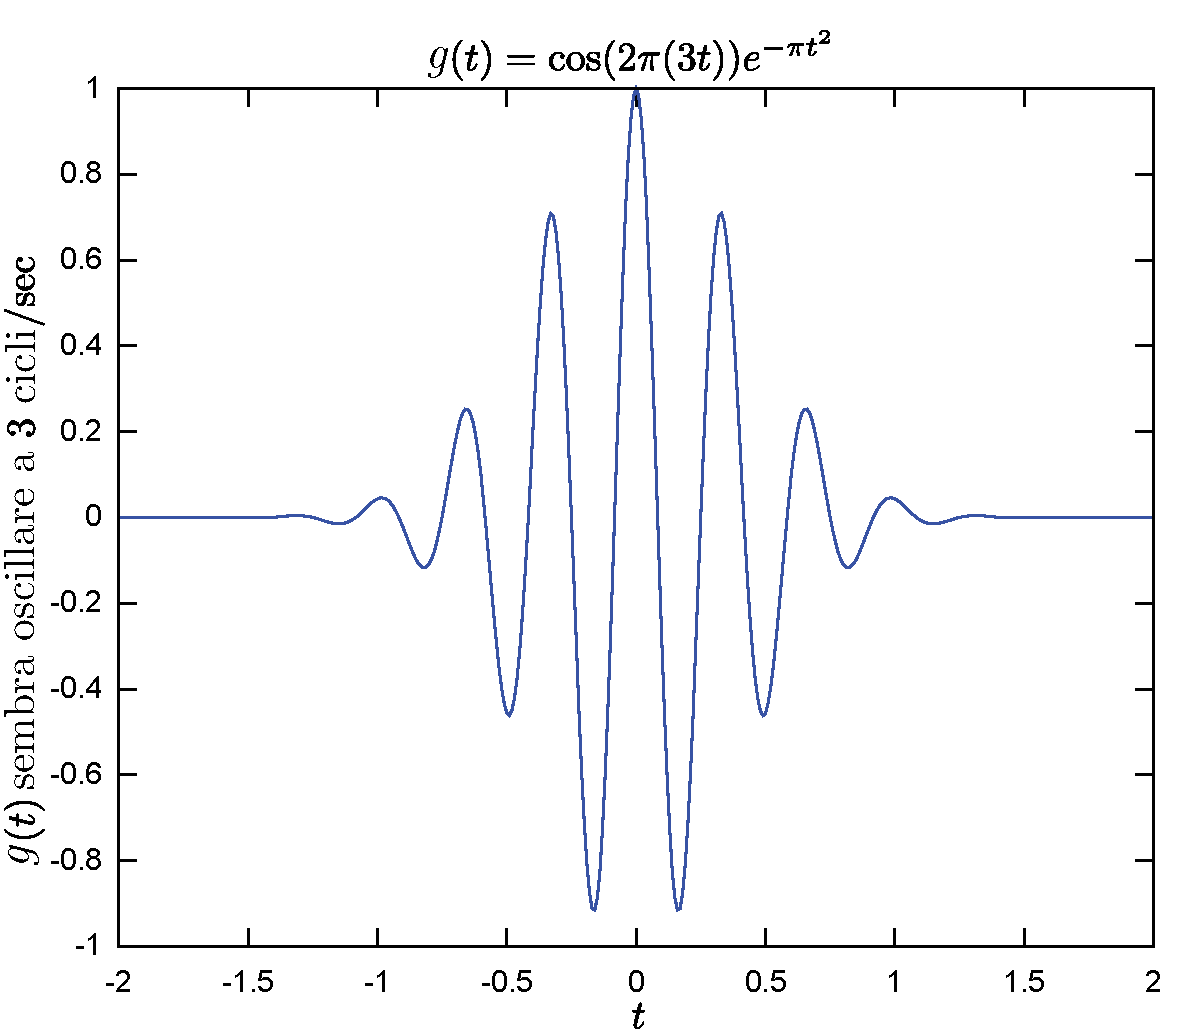
\includegraphics[trim=0cm 0cm 0cm 0cm, clip, scale=0.55]{images/fourier1.pdf}
\end{center}
\begin{center}
	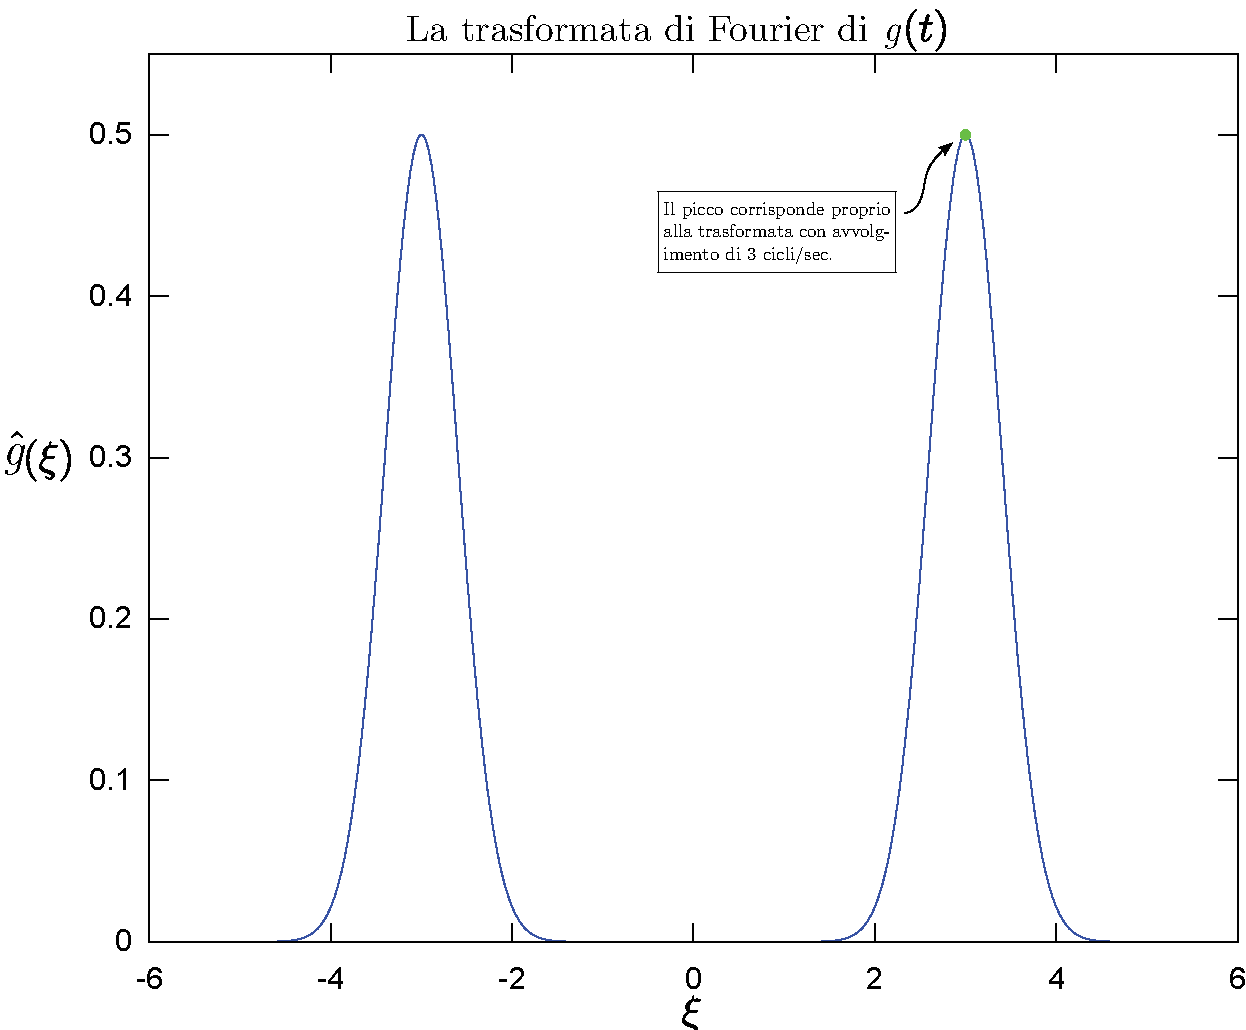
\includegraphics[trim=0cm 0cm 0cm 0cm, clip, scale=0.55]{images/fourier2.pdf}
\end{center}
Se studiamo i massimi della trasformata di Fourier di $g$ possiamo ricavare tutte le frequenze che la costituiscono, proprio come desiderato!\\
Questa che abbiamo dato è solo un'infarinatura molto generale del tema; per un approfondimento visivo particolarmente curato rimandiamo al video di \textbf{3Blue1Brown}, 	\textit{‘‘But what is the Fourier Transform?  A visual introduction.''} (\textcolor{redill}{\url{https://www.youtube.com/watch?v=spUNpyF58BY}}).
